\chapter{Problemløsning}\label{ch:chlabel}
I dette kapitel vil løsningen til problemformuleringen blive beskrevet og argumenteret for. Der bliver stillet krav til programmet for at løse problemet på den bedste måde. Ud fra disse krav vil der blive designet et program som løsning på problemformuleringen. Til sidst forklares det, hvordan dette design er implementeret, gennem programmeringen og datastrukturen. Der gives også beskrivelser og forklaringer af flere af de centrale funktioner fra kildekoden. 

% Ret eller omformuler endelig hvis du har noget bedre
% det hvordan et program kan blive til en løsning, på det problem der er opstillet i problemformuleringen. Først ved at formulerer et antal konkrete krav til løsningen. Efterfølgende designes der et program ud fra disse krav. Til sidst forklares det hvordan dette design er implementeret, ved at beskrive programmeringsstil og datastruktur. Der gives også beskrivelse og forklaringer af flere funktioner fra kildekoden.

\section{Krav til løsningen}
For at lave en funktionel løsning til projektets problemformulering, er det nødvendigt at opstille en række krav. Disse krav skaber rammen for de opgaver, løsningen skal være i stand til at udføre.\\
Et af de grundlæggende krav til løsningen er, at den skal være i stand til at opstille en stævneplan. Denne stævneplan skal overholde reglerne for stævner i Kidzliga floorball, som er stillet af Floorball Danmark \cite{kidzRegler}. Derfor er det nødvendigt at tage disse regler i betragtning, når en stævneplan bliver udarbejdet.
\par
I dette afsnit er de relevante regler beskrevet i rækkefølge efter prioritet. Prioriteringen bestemmer hvilke regler, der er vigtigst at overholde, og hvilke der kan undlades i tilfælde af, at det ikke er muligt at implementere dem alle.
\begin{itemize}
    \item \textit{En kamp varer seks minutter,\ og der skal være en til to minutters pause mellem hver kamp.} I forbindelse med projektet er det besluttet at sætte et krav om to minutters pause mellem hver kamp, da det er mere specifikt.
    \item \textit{Alle hold, der deltager, skal have cirka seks kampe.} Reglerne er i dette tilfælde heller ikke specificeret yderligere. Derfor er kravet i projektet gjort mere specifikt, ved at hvert hold skal have seks kampe. Kun hvis dette ikke er muligt, må et eller flere hold spille én kamp mere eller mindre. 
    \item \textit{Alle kampe i en runde skal startes og afsluttes på samme tid.} Denne regel er med til at sikre, at kampprogrammet ikke skrider så meget, at et hold pludselig skal spille to steder på samme tid, eller meget kort tid efter hinanden, hvilket strider imod den følgende regel.
    \item \textit{Alle hold skal have mindst én hvilekamp mellem hver kamp}, hvis det er muligt. Er det ikke muligt at indlægge en hvilekamp, tilstræbes det ifølge reglerne, at holdet, der spiller flere runder i træk, spiller på samme bane. I dette projekt er det fastsat som en regel, at kampen skal foregå på samme bane, i tilfælde af at en hvilekamp ikke er mulig. 
    \item \textit{Et hold må kun spille mod et andet hold, der er på det samme niveau.} Der er defineret fire forskellige niveauer i Kidzliga: N, A, B og C. Niveauerne er delt op, C er det højeste niveau, så kommer B, A og til sidst N, som står for nybegynder. 
    \item Det kan forekomme, at et kampprogram bliver hængt op i en hal, hvor stævnet bliver afviklet. Derfor stilles der et krav til løsningen, om at \textit{det udviklede kampprogram skal være opstillet på en præsentabel måde.} Det er herudfra bestemt, at opdeling i runder skal fremstå tydeligt, hvor hver runde er opdelt i kampe. Her skal banenummer, niveau og startstid for hver runde også stå.
\end{itemize} 

Det er nødvendigt at overholde disse specifikke regler, da problemet er afgrænset til Kidzliga. Ydereligere, opstilles krav til løsningen, som ikke er direkte stillet af Floorball Danmark. Disse regler fremsættes for at øge kvaliteten af stævneplanen. Et menneske vil naturligt følge dem, men reglerne skal defineres klart, for at et program også overholder dem.
\begin{itemize}
    \item \textit{Et hold må ikke spille mere end 2 kampe i træk.} Dette er en udvidelse af reglen, om at der skal være en hvilkekamp mellem hver kamp og gælder, når dette ikke kan lade sig gøre. 
    \item \textit{Hvert hold skal spille mod et andet hold igen, så få gange som muligt, og to hold må ikke spille mod hinanden to kampe i træk.} Dette er besluttet for at sikre, at hvert hold kommer til at spille med så mange forskellige andre hold som muligt.
\end{itemize}
Disse regler skal overholdes for at få en stævneplan af høj kvalitet, men er ikke nødvendige at overholde for at få en fungerende stævneplan.
\\\\
Problemformuleringen nødvendiggør også et krav, om at stævneplanen skal være fleksibel. Det skal derfor være muligt at foretage ændringer i stævneplanen, efter den er blevet udarbejdet. Programmet skal tillade brugeren at tilføje og fjerne hold fra stævneplanen. Dette vil gøre stævneplanen mere fleksibel, da brugeren får mulighed for at lave hurtige ændringer i et allerede eksisterende kampprogram.
\\\\
Ud fra disse krav er det muligt at komme frem til en ide og et overordnet design til et program, som kan løse problemet. 

\section{Design}
Ud fra kravene er det muligt at designe et program til at løse problemstillingen. Designet er den overordnede ide, om hvordan programmet skal fungere og hænge sammen. Samtidigt afklarer designet, hvordan problemet kan deles op i flere, mere overkommelige opgaver, for at gøre det nemmere at udvikle og forstå programmet. 
\\\\
Der er blevet lavet tre flowcharts til at beskrive programmets design. \textit{Det overordnede flowchart} viser strukturen af programmet (figur \ref{fig:overordnet-flowchart}). \textit{Lav ny stævneplan} (figur \ref{fig:lav-flowchart}) viser tanken bag, hvordan programmet laver en stævneplan. Til sidst er der \textit{rediger stævneplan} (figur \ref{fig:rediger-flowchart}), som viser, hvordan programmet skal kunne tilføje og fjerne hold fra en eksisterende stævneplan. Det overordnede flowchart bliver gennemgået først.

\begin{figure}[H]
  \centering
  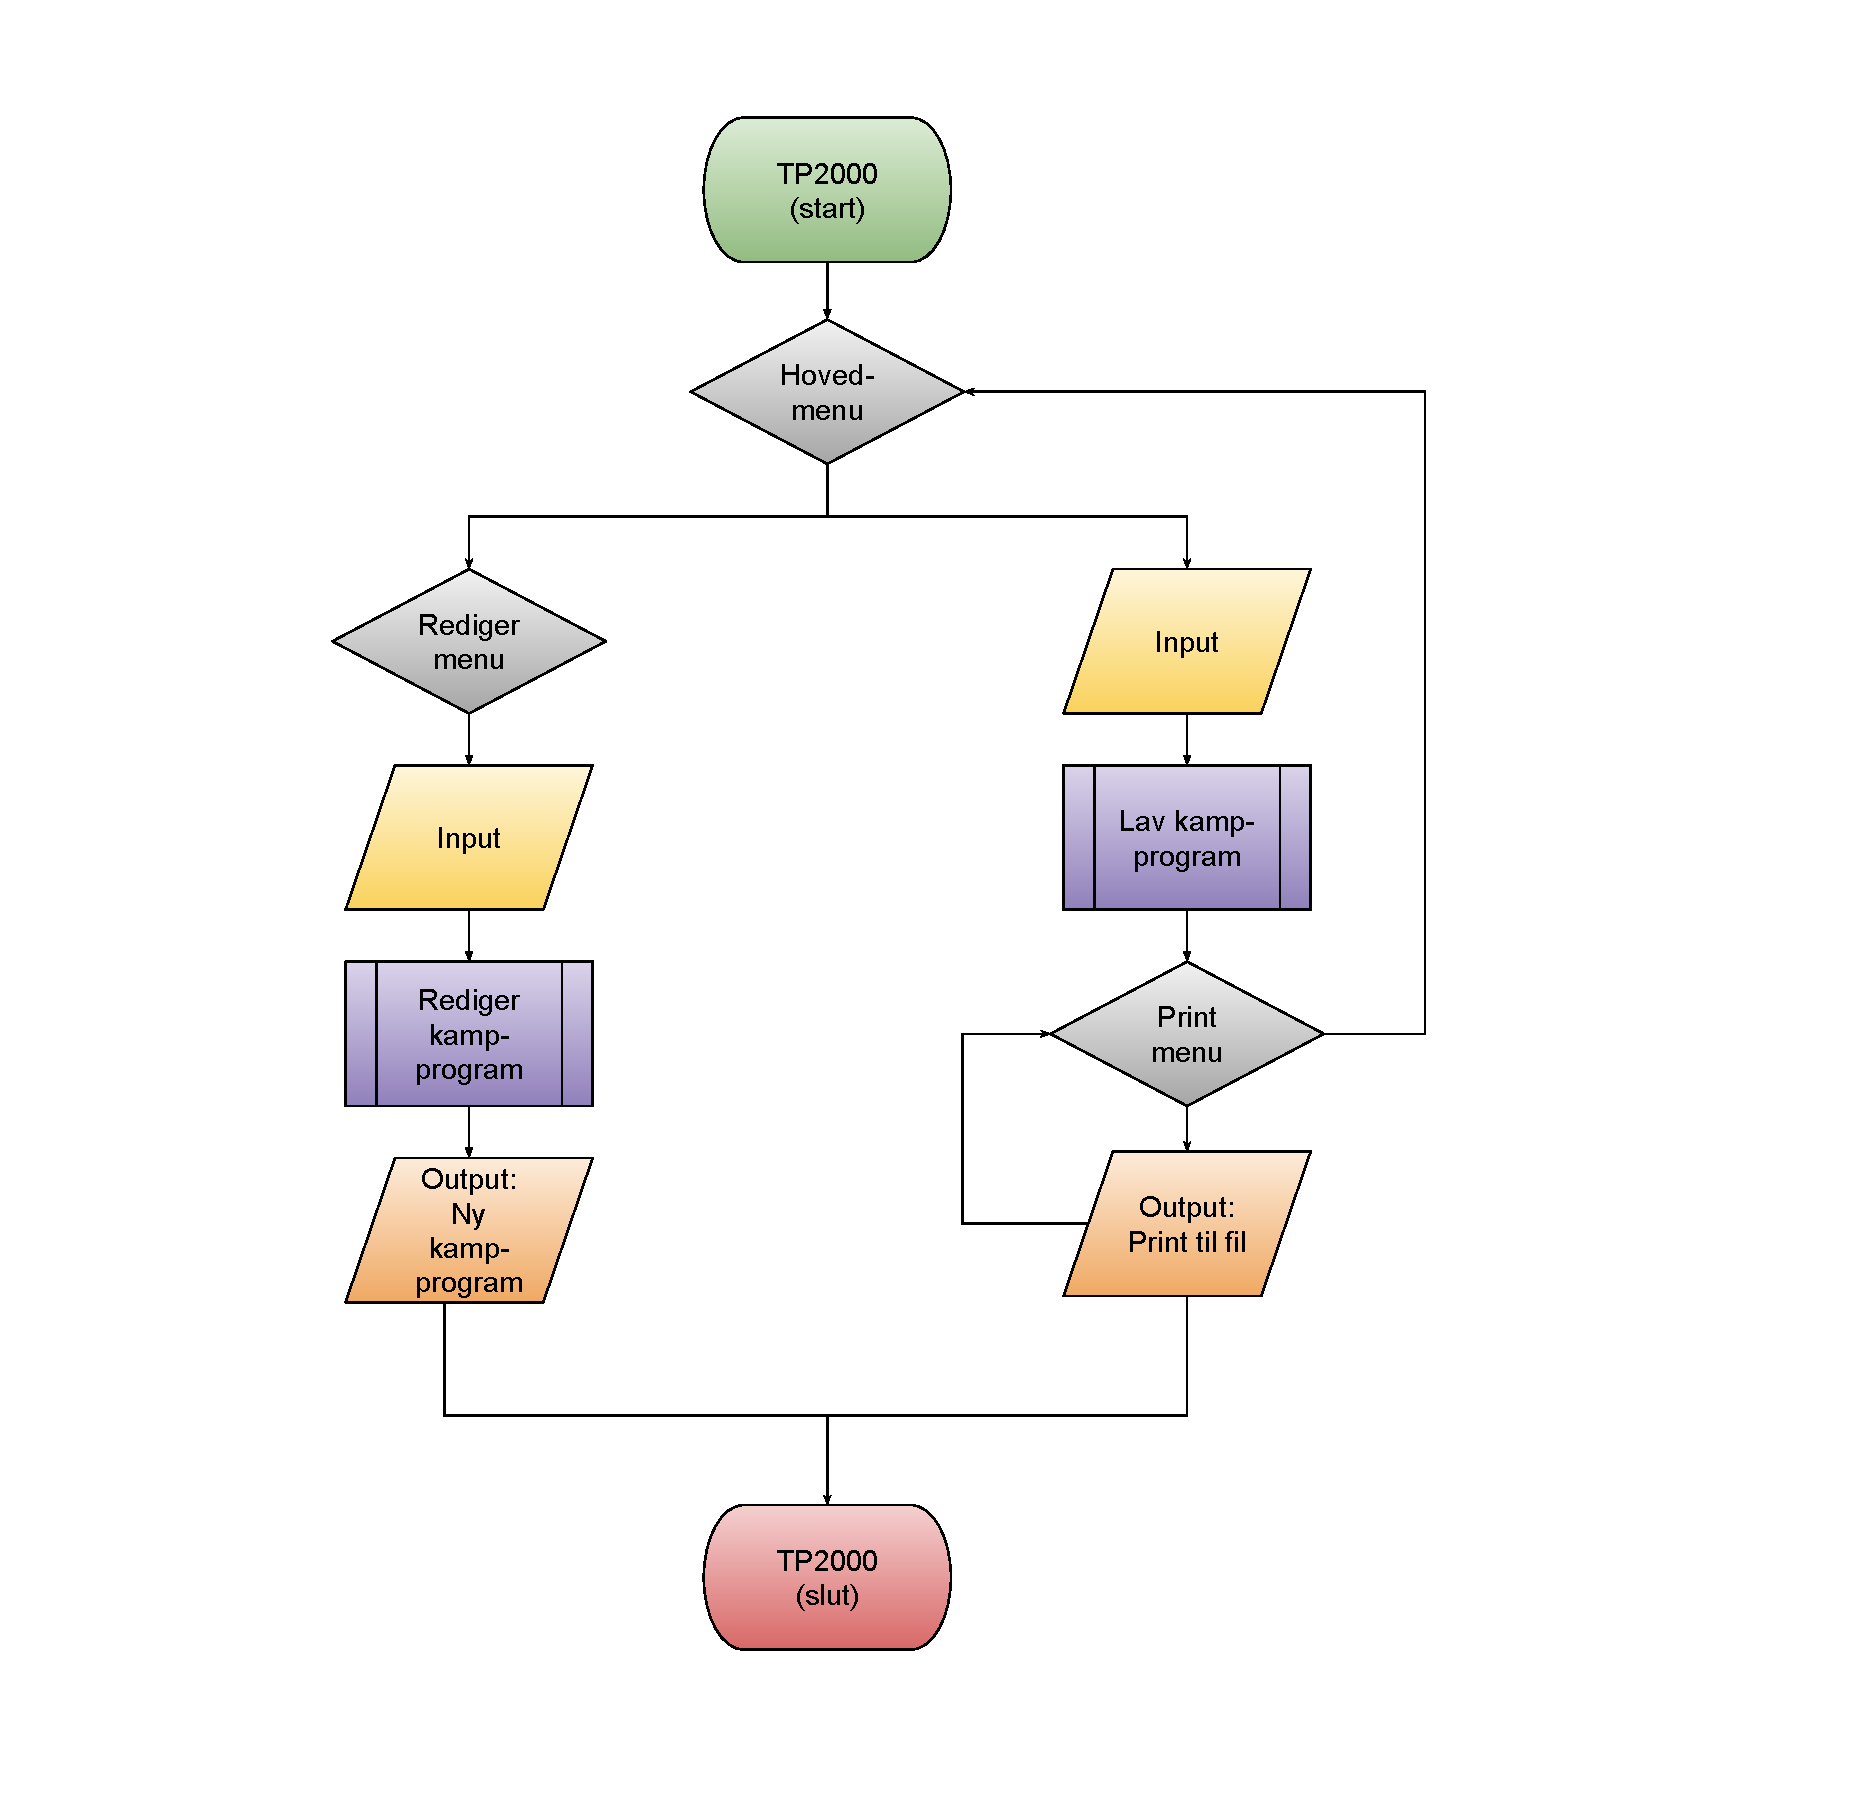
\includegraphics[width=0.9\textwidth]{figures/Overordnet.pdf}
  \caption{Flowchart over programmets overordnede struktur.}
  \label{fig:overordnet-flowchart}
\end{figure}

På figur \ref{fig:overordnet-flowchart} ses den overordnede struktur over programmets opbygning. Programmet starter med en hovedmenu, hvor brugeren skal vælge mellem to hovedgrene. Den højre gren (figur \ref{fig:lav-flowchart}) giver mulighed for at lave en ny stævneplan, og den venstre gren (figur \ref{fig:rediger-flowchart}) giver mulighed for at redigere en allerede eksisterende stævneplan. Disse valgmuligheder er med til at give et overblik over hvad programmet kan, og giver mulighed for at brugeren selv kan bestemme hvad de ønsker at gøre med programmet.

\subsubsection{Lav ny stævneplan}
For at løsningen skal være i stand til at overholde de opstillede krav for oprettelse af en stævneplan, har programmet brug for følgende informationer fra brugeren:
\begin{itemize}
    \item Holdnavne med niveau i en tekstfil
    \item Antal baner
    \item Starttidspunktet for stævnet
\end{itemize}
Disse informationer er nødvendige at have for at kunne lave en stævneplan, der er opstillet ordentligt og korrekt i overensstemmelse med de andre krav og regler. 
\par
Holdnavne og niveauer indlæses fra en tekstfil, da der kan være mange hold, og brugeren kan miste overblikket, hvis input tastes gennem terminalen. Når holdnavne skrives ind på en fil, bliver det mere overskueligt for brugeren. Dette kræver dog en specifik opsætning af filen, da programmet ellers ikke vil kunne læse den.
\\\\
% Beskrivelse af opsætningen
I eksemplet nedenfor fremstår det, at kravene til opsætningen er, at der skal være ét holdnavn på hver linje efterfulgt af et komma og holdets niveau. Holdnavnet må indeholde visse specialtegn (såsom "?!/\%-\_"\ mm.), men det første tegn skal være et bogstav. Niveauet, der angives med et bogstav, må være både stort og småt.
\\\\
% Eksempel
\textbf{Holdnavn1, Niveau}\\
\textbf{Holdnavn2, Niveau}\\
\textbf{...}\\

Antallet af baner og starttidspunktet indlæses gennem terminalen, da disse er hurtigere for brugeren at taste ind.
\par
Herefter sammensættes stævneplanen. Dette sker ved brug af tilfældig sammensætning af kampe og runder, hvorefter hver runde evalueres, og der tælles fejl, i forhold til hvor mange gange de højest prioriterede regler er blevet brudt. Hvis runden ingen fejl har, godkendes den, ellers bliver den sammensat anderledes, indtil den er acceptabel. Hvis der ikke kan findes en rundesammensætning, som overholder de opstillede regler, startes processen igen fra første runde.
\par
Der var en overvejelse om at sammensætte stævneplanen på en struktureret måde, som en imitation af hvordan et menneske ville lægge planen, men gøre det hurtigere end en person kunne gøre det. Med denne metode er der dog en risiko, for at den bedste stævneplan ikke bliver fundet, da alle muligheder ikke nødvendigvis bliver udforsket. Ved at bruge den tilfældige metode, er der mulighed for at få sammensat flere forskellige stævneplaner tilfældigt, hvor den mest optimale udvælges.
\par
For at få det optimale resultat vil der være behov for et point-system, som giver point i forhold til de regler, der ikke er givet af Floorball Danmark. Jo flere regler der bliver opfyldt, jo flere point får stævneplanen. Hver stævneplan bliver hermed sammenlignet med den hidtil mest optimale, og den med flest point bliver gemt. Efter et fastsat antal iterationer bliver den bedste printet ud (se afsnit \ref{implementering}).
% \par
% Projektets program giver mulighed for at gøre dette, men det kan tage noget tid for programmet at komme frem til den bedste stævneplan. Dette skyldes, at for at stævneplanen bliver god nok, skal programmet køres et bestemt antal gange, som er meget stort, i forhold til den tid det tager for programmet at komme med en god stævneplan. Der er derfor også mulighed for at få lavet en stævneplan hurtigt, men hvor den ikke har lige så høj kvalitet som den anden mulighed.

% Det er dog ikke det projektets program gør, da denne løsning vil tage for lang tid for programmet at komme frem til den bedste stævneplan. Dette skyldes at for at stævneplanen bliver god nok, skal programmet køres et bestemt antal gange, som er for stort i forhold til den tid det tager for programmet at komme med en god stævneplan.

\begin{figure}[H]
  \centering
  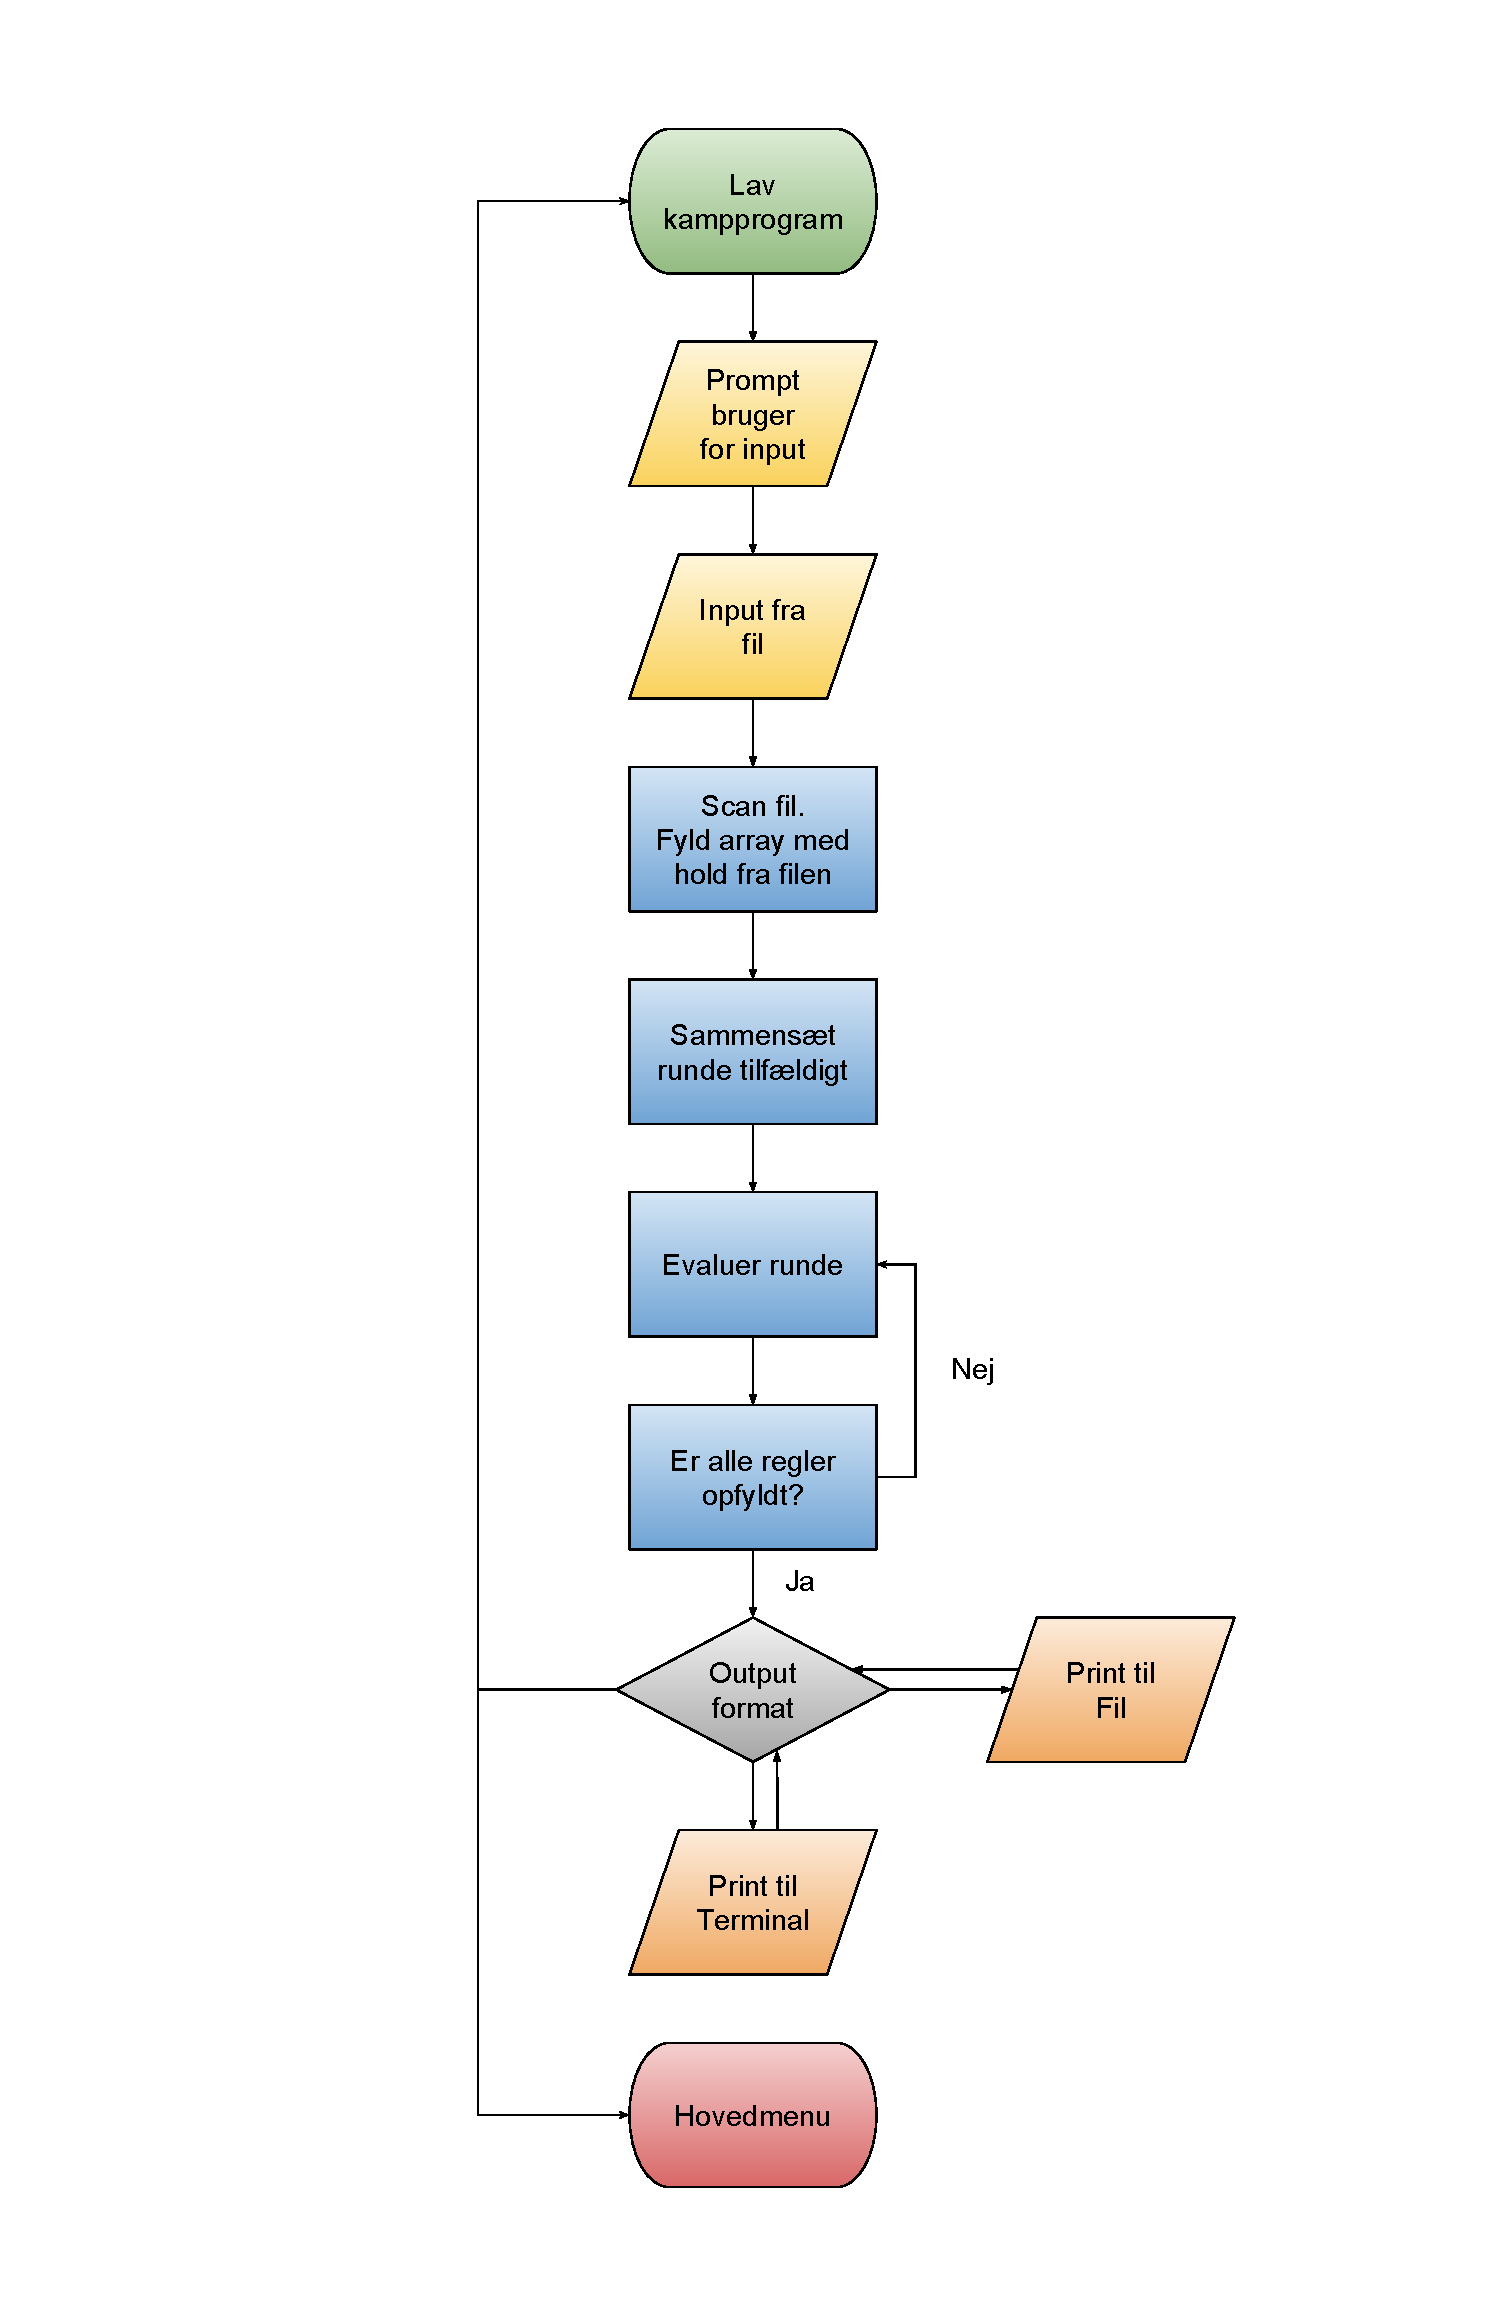
\includegraphics[width=0.7\textwidth]{figures/Lavflowchart.pdf}
  \caption{Flowchart over processen for at lave et kampprogram}
  \label{fig:lav-flowchart}
\end{figure}

Når en stævneplan skal sættes op, bliver brugeren bedt om at foretage et valg om hvilket output, der ønskes. Dette kan ses på figur \ref{fig:lav-flowchart}. Her er det muligt at få stævneplanen printet til terminalen, så brugeren har mulighed for at tjekke stævneplanens sammensætning, for at se om det er acceptabelt. Hvis brugeren ikke er tilfreds, kan der sammensættes en ny stævneplan fra hovedmenuen. Brugeren kan også få printet stævneplanen ud på en fil, da det er et krav, at man skal kunne printe stævneplanen ud og hænge den op i hallen.\\
Når brugeren er færdig med at lave stævneplanen, kommer de tilbage til hovedmenuen, hvor der igen er mulighed for at vælge mellem de to grene på figur \ref{fig:overordnet-flowchart}.

\subsubsection{Rediger stævneplan}
Hvis brugeren vælger at redigere stævneplanen, følger man venstre hovedgren på figur \ref{fig:overordnet-flowchart}. Som det fremstår på det overordnede flowchart, gør løsningen det muligt for en bruger at redigere en allerede eksisterende stævneplan ved at tilføje eller fjerne hold. For at dette kan lade sig gøre, kræves det, at den eksisterende stævneplan er af samme format som programmet bruger.
% Indsæt rediger-kampprogram flowchart her!
\begin{figure}[H]
  \centering
  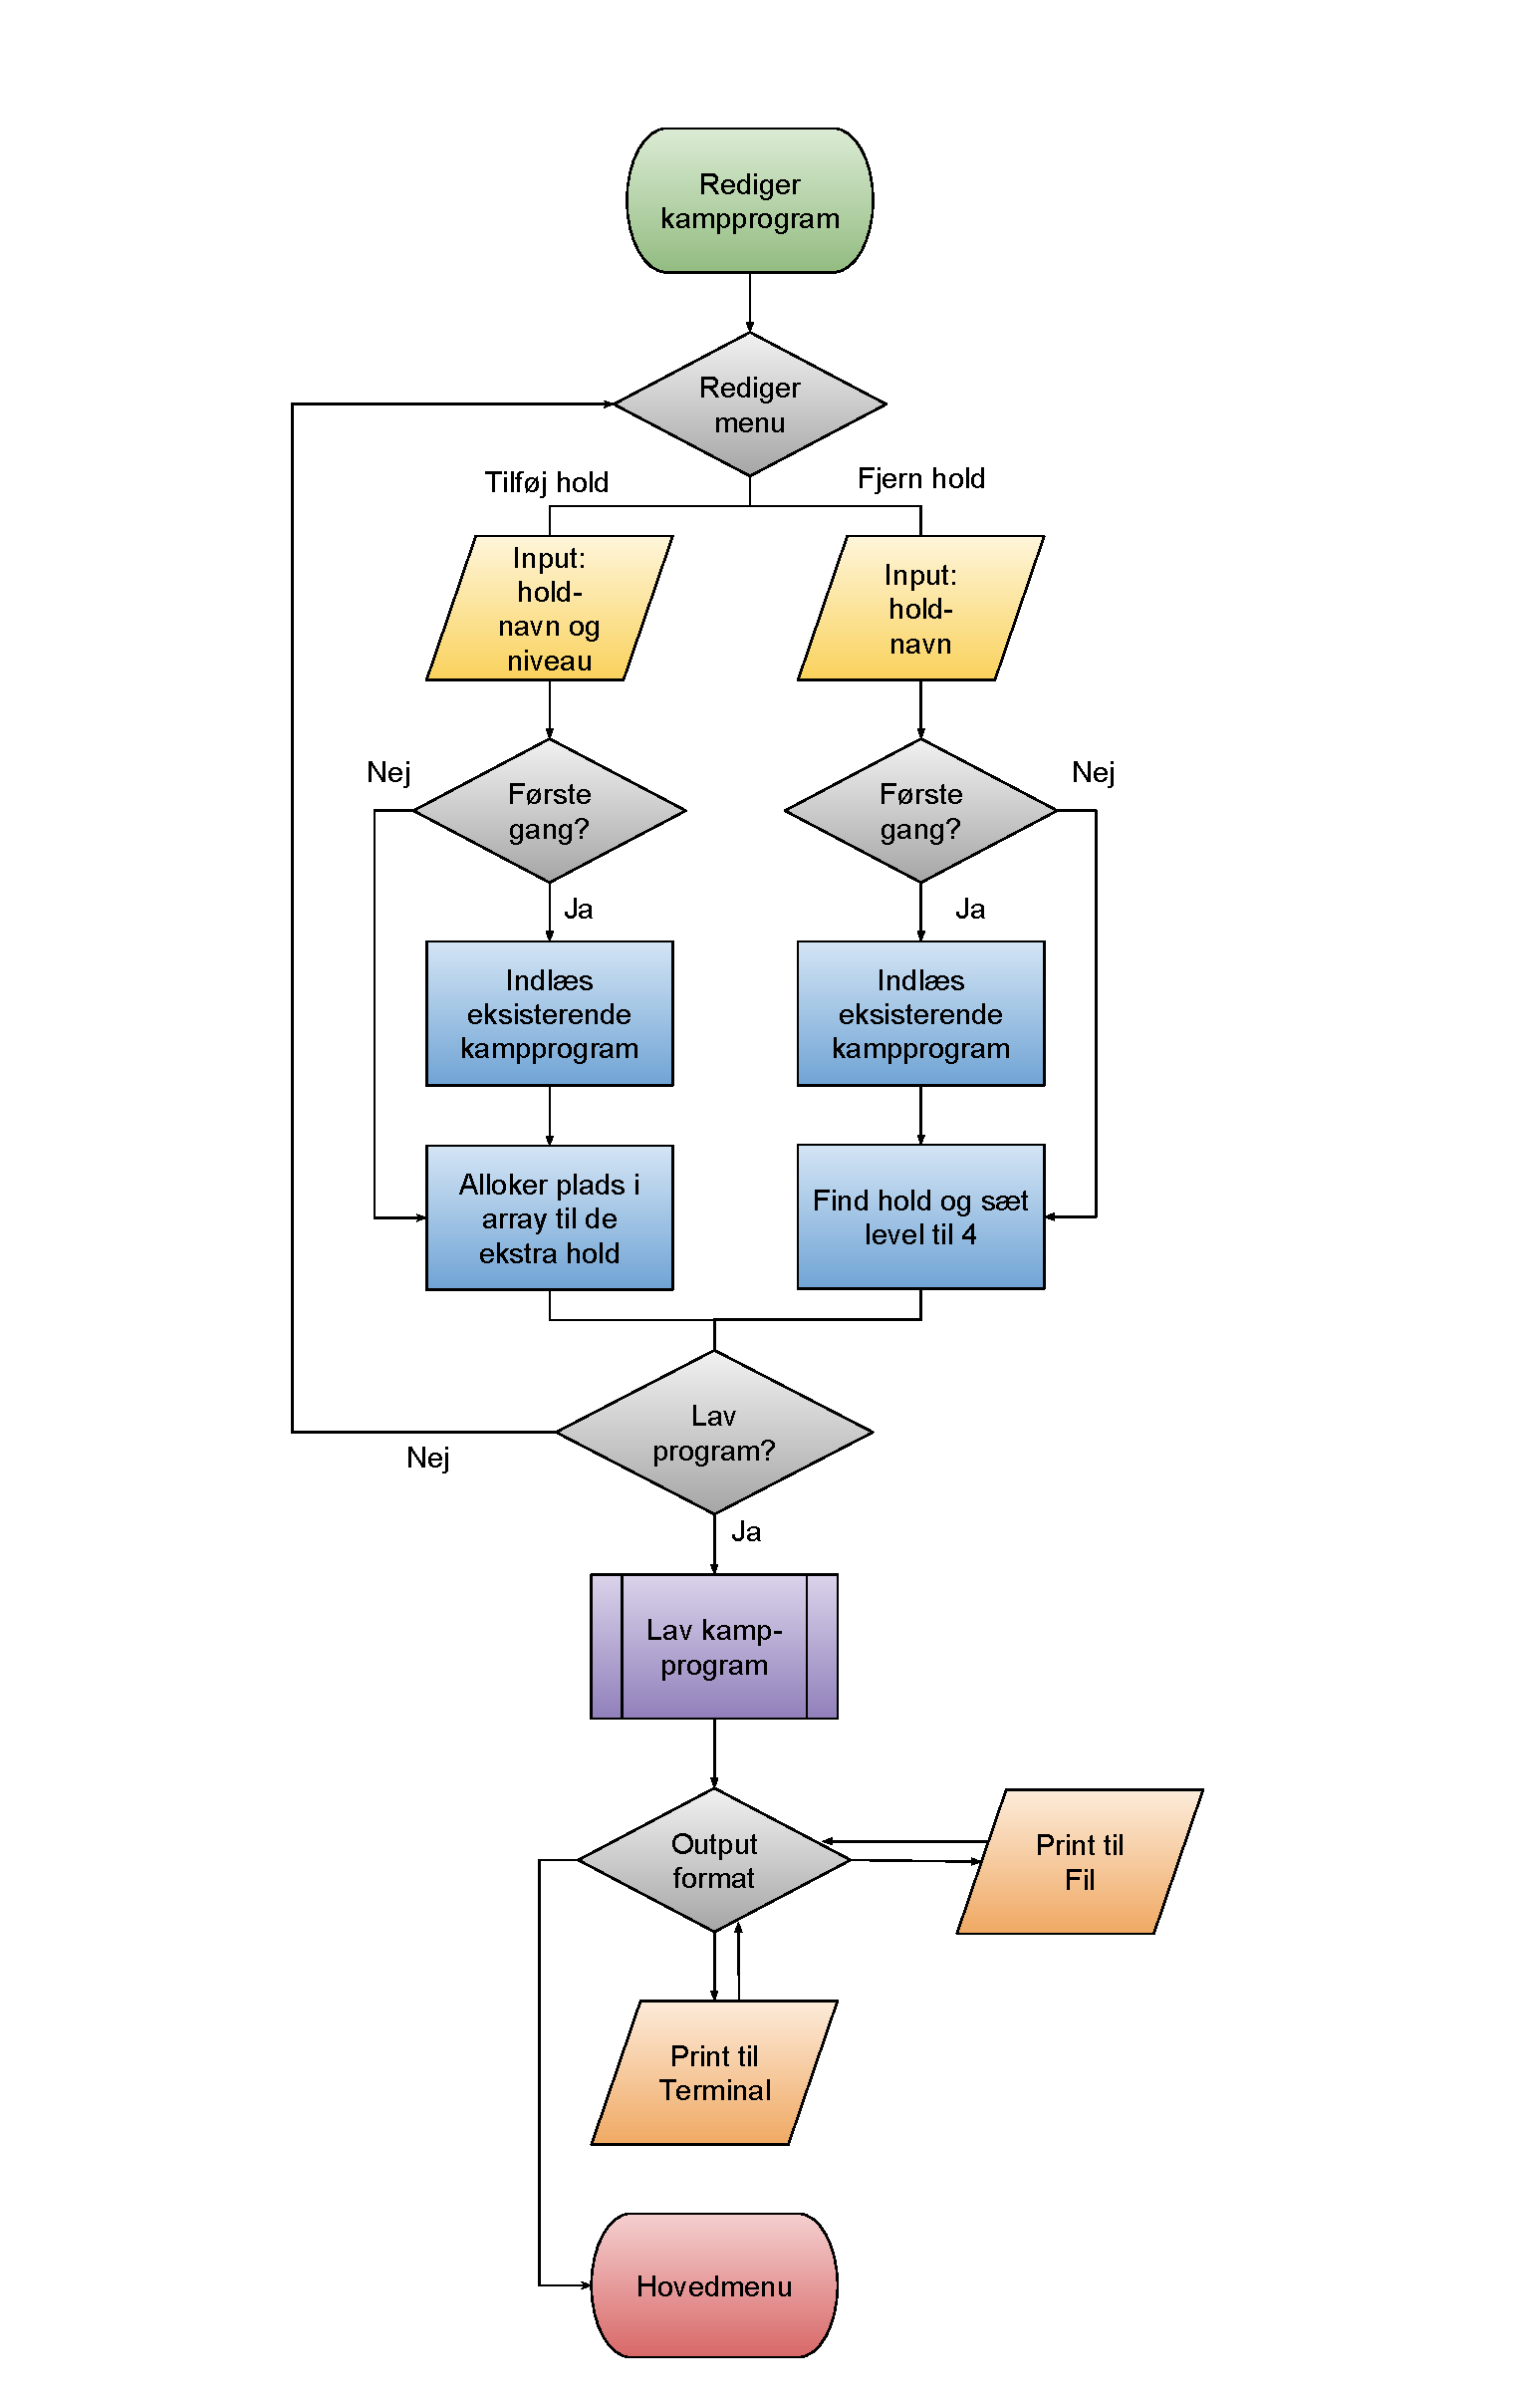
\includegraphics[width=0.7\textwidth]{figures/Redigerflowchart.pdf}
  \caption{Flowchart over processen for at redigere et kampprogram.}
  \label{fig:rediger-flowchart}
\end{figure}
% % % % % % % % % % % % % % % hest?
Måden hvorpå programmet redigerer en eksisterende stævneplan, er illustreret på figur \ref{fig:rediger-flowchart}. Først skal brugeren indtaste hvilke hold der skal tilføjes eller fjernes. Efterfølgende indlæses informationerne fra en fil med den eksisterende stævneplan. Dette skal dog kun gøres én gang inden der foretages ændringer. Efterfølgende kan der foretages flere ændringer, indtil brugeren er tilfreds. 
\par
Herefter bearbejdes informationerne om holdene, så de stemmer overens med de ændringer, brugeren ønsker. Dette kan ses i kildekode \ref{code:updateTournament} side \pageref{code:updateTournament}. Til sidst fremstilles en stævneplan med ændringerne, på samme måde som der fremstilles en ny stævneplan. Brugeren har mulighed for at printe stævneplanen, enten i terminalen eller til en fil. I terminalen kan stævneplanen inspiceres, og der er mulighed for at lave yderligere ændringer eller generere en ny stævneplan, før den færdige plan gemmes.

\section{Implementering}\label{implementering}
% Hvilke antagelser der er i forhold til at programmet skal kører ordentligt.
% Hvordan gør vi rent faktisk det her, helt nede i koden
% Forklaring af snippets
Dette afsnit handler om implementeringen af løsningen. Den måde koden er skrevet, tager udgangspunkt i det design, der er beskrevet i forrige afsnit. Den anvendte programmeringsstil beskrives ligeledes for nemmere at kunne læse kildekoden. Datastruktureren, der er brugt i kildekoden, forklares, og der argumenteres for trufne valg i denne forbindelse. Til sidst beskrives de mest centrale funktioner fra kildekoden, med tilhørende forklaringer og kodeeksempler. Dette gøres for at hjælpe læseren med at følge de tanker og ideer, der har været bag de valg, som er blevet truffet.

\subsection*{Programmeringsstil}
Som programmeringsstil refereres der til en modificeret version af C Coding Standard \cite{codingstyle}. En af de modifikationer der er foretaget, er at betingelser, i eksempelvis if-else kæder, har konstanten placeret til højre i stedet for til venstre, som standarden anbefaler. Et eksempel på dette kan ses i kodeeksempel \ref{code:conditionStyle} herunder.

\begin{listing}[H]
\begin{minted}[frame=lines, framesep=3mm, baselinestretch=1, linenos, bgcolor=LightGray]{c}
/* Som standarden foreskriver: */
if (0 == var) {
    ...
}

/* Som det gøres i dette projekt: */
if (var == 0) {
    ...
}
\end{minted}
\captionof{listing}{Kodeeksempel på forskelle mellem opsætningen af kontrolstrukturer, ifølge C Coding Standard \cite{codingstyle} og dette projekt.}
\label{code:conditionStyle}
\end{listing}

Derudover skrives kommentarer ikke i slutningen af eksempelvis en if-else kæde, som det er beskrevet i C Coding Standard. I stedet skrives disse i begyndelsen eller ved siden af (kodeeksempel \ref{code:commentStyle}). Dette gøres så forklaringen kommer før koden for at øge læsbarheden.

\begin{listing}[H]
\begin{minted}[frame=lines, framesep=3mm, baselinestretch=1, linenos, bgcolor=LightGray]{c}
if (var == 0) {
    ...
} /* Som standarden foreskriver: */


/* Som det gøres i dette projekt: */
if (var == 0) {
    ...
    ...     /* Dette gøres også */
}
\end{minted}
\captionof{listing}{Kodeeksempel på forskelle mellem placering af kommentarer ifølge C Coding Standard \cite{codingstyle}, og dette projekt.}
\label{code:commentStyle}
\end{listing}

Det tilstræbes, at antallet af tegn per linje er 78 \cite{codingstyle}, da koden skal kunne passe på en A4-side. Der accepteres dog visse brud på denne regel i kildekoden. Dette skyldes, at nogle af programmets funktioner har mange parametre, og dermed overskrider de 78 tegn. 
\par
I kildekoden, er input, output og kommentarer skrevet på dansk, mens alt andet er skrevet på engelsk.
% Dette er ikke alle afvigelser

\subsection*{Datastruktur}
Udover en fast programmeringsstil i programmet, er der også opsat en fast datastruktur. Dette gøres, da det så bliver muligt at arbejde med problemet på en mere intuitiv og overskuelig måde. I dette afsnit, vil denne datastruktur blive beskrevet.
\par
Strukturen af Kidzliga stævner abstraheres i kildekoden til en samling af \textbf{\textit{match}} structs, der hver repræsenterer en kamp. Hver af disse indeholder ligeledes en \textbf{\textit{team}} struct for hvert hold i kampen. Stævnet er sat op som et array af \textbf{\textit{match}} structs, der hver tildeles en bane og kan deles ind i runder. Niveauet bliver repræsenteret som et bogstav, men bliver reelt set behandlet som heltal, og derfor er det lavet til en enumeration type \textbf{\textit{levels}}.\\
Disse bliver gennemgået i de næste tre afsnit.

%Strukturen af Kidzliga stævner abstraheres i kildekoden til en samling af flere kampe, der er grupperet i runder. Der afvikles én kamp per bane i hver runde, og en kamp er en \textbf{\textit{match}} struct, der består af to hold som er \textbf{\textit{team}} structs, af samme niveau. 

\subsubsection{Team struct}
En instans af \textbf{\textit{team}} structen (kildekode \ref{code:teamStruct}) indeholder al den information, der er relevant i forbindelse med et enkelt hold i et stævne. \\
Informationen er fordelt på structens members, der består af en streng med holdets navn, et heltal med antallet af kampe de har spillet og et heltal med holdets niveau.\\
Heltallet \textbf{\textit{games}} bruges til at holde styr på, at et hold spiller det rette antal kampe. Dette tal skal tælles op hver gang de bliver sat i en ny \textbf{\textit{match}}.

\begin{listing}[H]
\begin{minted}[frame=lines, framesep=3mm, baselinestretch=1, linenos, bgcolor=LightGray]{c}

typedef struct {
  char team[MAX_NAME_LEN];
  int games;
  int level;
} team;

\end{minted}
\captionof{listing}{Structen team, som den er defineret i kildekoden}
\label{code:teamStruct}
\end{listing}

\subsubsection{Match struct}
Structen \textbf{\textit{match}} (kildekode \ref{code:matchStruct}) indeholder den information, der er relevant for en kamp. Informationen er, ligesom tidligere, fordelt på de enkelte members, der består af en \textbf{\textit{team}} struct med det ene hold i kampen, en \textbf{\textit{team}} struct med det andet hold i kampen, et heltal med niveauet for kampen og et heltal, der repræsenterer banen, hvorpå kampen afvikles. \\
De members, der indeholder de deltagende hold, er af den tidligere nævnte type \textbf{\textit{team}}. Dette gør det muligt at få adgang til information om holdene, der deltager i en given kamp, ved at tilgå disse instansers members.

\begin{listing} [H]
\begin{minted}[frame=lines, framesep=3mm, baselinestretch=1, linenos, bgcolor=LightGray]{c}

typedef struct{
  team team_a;
  team team_b;
  int level;
  int field;
} match;

\end{minted}
\captionof{listing}{Structen match, som den er defineret i kildekoden}
\label{code:matchStruct}
\end{listing}

\subsubsection{Enumeration type}
Udover disse structs er der også defineret en enumeration type ved navn \textbf{\textit{levels}} (kildekode \ref{code:levelEnum}). Grunden til dette er, at niveauerne, som de defineres i de officielle regler, er bogstaver. For at gøre det lettere at arbejde med i kildekoden kan disse bogstaver igennem denne enumeration type, konverteres til heltal. \\
Der er en værdi yderligere i enumeration typen ved navn EMPTY. Dette er nødvendigt for redigeringsdelen, da holdene struktureres i et array, hvor det ikke er muligt at slette et hold fra. Brugen af arrayet vil blive uddybet senere i afsnittet. Hvis et element i dette array er "tomt", bliver holdets niveau sat til denne værdi, så de kan udelades når stævneplanen sammensættes.

\begin{listing}
\begin{minted}[frame=lines, framesep=3mm, baselinestretch=1, linenos, bgcolor=LightGray]{c}

enum levels {EMPTY, N, A, B, C};

\end{minted}
\captionof{listing}{Enumeration typen levels, som den er defineret i kildekoden. Denne er ikke typedefined, da typen ikke benyttes direkte i koden.}
\label{code:levelEnum}
\end{listing}

Datastrukturen, der gøres brug af i dette projekt, består ikke kun i definitionen af nye datatyper. Selve stævnet, der som sagt består af en samling af kampe, er i kildekoden opstillet som et array med elementer af typen \textbf{\textit{match}}. Dette har til formål at samle alle kampene, så de er lette at overskue og arbejde med. Dette array er struktureret i rækkefølge, efter hvornår hver kamp finder sted. Denne struktur gør det muligt at udregne, hvilke kampe der er i hver runde, da der i hver runde spilles én kamp på hver bane. Derfor er det muligt at regne antallet af runder ud, hvis man kender antallet af baner, og det samlede antal kampe. Det er på en lignende måde muligt at udregne hvilken runde, en specifik kamp afvikles i (se afsnit \ref{?}). Derfor er det ikke nødvendigt at opstille data efter runder.
\par
Ligeledes er alle holdene der deltager i stævnet, samlet i et array, med elementer af typen \textbf{\textit{team}}.
\par
Når der i kildekoden arbejdes med et af de arrays, som er beskrevet ovenfor, eksempelvis i en funktion, sendes antallet af aktuelle elementer også med. Dette gør det lettere at arbejde med disse arrays, da det ikke er muligt at finde frem til størrelsen, når et array bruges i en funktion. Dette skyldes at der sendes en pointer til arrayet som inputparamenter, og ikke selve arrayet. Man ville derfor kunne finde størrelsen på denne pointer, men ikke størrelsen på arrayet.
\\\\
Disse datastrukturer bliver brugt gennem hele koden og er måden, information bliver sendt rundt mellem de forskellige funktioner, som man kan se i selve kildekoden.

\subsection*{Udvalgte eksempler på kildekode}
I dette afsnit bliver der gennemgået forskellige udsnit af kildekoden i programmet. Denne kildekode vil blive forklaret, og der vil blive argumenteret for de valg, der er blevet taget under programmeringen.
\par
Programmet er lavet ud fra visse antagelser, om forholdene i stævnet. En af dem er, at der mindst er 10 hold i hvert niveau. Denne antagelse er nødvendig for, at et hold ikke kommer til at spille mod de samme modstandere for ofte. Desuden vil programmet ikke fungere optimalt hvis der er under 10 hold, da der ikke vil være nok mulige sammensætninger, og hvert hold må spille maks seks kampe.
\\
Der er også placeret en restriktion på hvor mange baner, der maksimalt er tilladt, da det bliver en udfordring for programmet at sammensætte en korrekt stævneplan, hvis der er for mange baner.
\\
På baggrund af disse antagelser bliver funktionen createNewTournament først beskrevet, da denne funktion skal køres først for at lave den første stævneplan.

\subsubsection{createNewTournament}
I dette afsnit gennemgås \textbf{\textit{createNewTournament}}-funktionen med forklaringer og argumenter for den valgte implementering (kildekode \ref{code:createNewTournament}). Når brugeren i hovedmenuen vælger at lave en ny stævneplan, indhenter programmet antallet af baner, starttidspunktet for stævnet og navnet på input-filen fra brugeren. Denne fil skal indeholde en liste af holdnavne med tilhørende niveauer. Filen scannes to gange i løbet af funktionen. Først scannes den for at få antallet af hold, som også svarer til antal linjer, der ikke er tomme, i filen (l. 29).
\par
\textbf{\textit{Number\_of\_matches}} udregnes herefter, fordi det er nødvendigt for at udregne antallet af runder, der skal være i stævneplanen. Da der i kravene står, at hvert hold skal spille ca. 6 kampe, vil udregningen se således ud:
\[\frac{6\ * \ number\_of\_teams}{2}\]
Der divideres med 2, da hver kamp indeholder to hold, og derfor tælles dobbelt i forhold til udregningen af antallet af kampe. (l. 32)
\par
Funktionen \textbf{\textit{getNumberOfRounds}} (l. 33) udregner antallet af runder, \textbf{\textit{number\_of\_matches}} svarer til. Da der regnes med heltal, vil decimaltal blive rundet ned, når der divideres. Dette er dog ikke hensigtsmæssigt i forhold til udregningen, da der i nogle tilfælde vil mangle en runde. Funktionen undersøger derfor om $number\_of\_rounds \\ mod(number\_of\_fields)$ er lig med nul eller ej. Hvis den er lig med nul, kan der divideres uden ekstra tilføjelser. Formlen vil hermed se således ud:
\[\frac{number\_of\_matches}{number\_of\_fields}\]
Hvis dette ikke er tilfældet, er der behov for at addere 1 til resultatet for at få den manglende runde med, og formlen vil derfor være:
\[\frac{number\_of\_matches}{number\_of\_fields} + 1\]
\\
Herefter allokeres der plads dynamisk til et array \textbf{\textit{all\_teams}}, som vil indeholde alle holdnavne (l. 38). Dette gøres gennem funktionen \textbf{\textit{allocateMemoryTeams}}, hvor der bruges malloc, da der ikke er behov for at nulstille elementerne i arrayet, før det bruges. Dette skyldes, at arrayets elementer alligevel bliver erstattet med holdnavne, så det er lige meget, hvad der tidligere var i det bestemte element. Opfyldningen af arrayet sker gennem \textbf{\textit{scanTeamFile}} funktionen, som scanner filen med holdnavnene for at kopier dem over i \textbf{\textit{all\_teams}}.
\\
Der bliver brugt dynamisk allokering fremfor statisk allokering, fordi størrelsen på arrayet afhænger af \textbf{\textit{number\_of\_matches}}, som ikke er et fast tal. \textbf{\textit{Number\_of\_matches}} beregnes ud fra \textbf{\textit{number\_of\_teams}}, som afhænger af antallet af holdnavne, der står i filen. 
\par
Der bliver også allokeret plads til \textbf{\textit{tournament}}-arrayet (l. 45). Dette array er, hvor de forskellige kampe vil blive sat ind, i den rækkefølge de vil fremkomme i den endelige fil for stævneplannen. Der er to måder, hvorpå arrayet kan fyldes op. Dette bestemmes af brugeren, da den ene måde er hurtigere end den anden, men hvor den anden har bedre kvalitet end den første. 
\par
Arrayet for den hurtige stævneplan fyldes gennem en do-while løkke, som kalder funktionen \textbf{\textit{checkTournament}}. Denne funktion kører en anden funktion, \textbf{\textit{createTournament}}, som har til formål at sætte en stævneplan sammen, sådan at de krav, der er fastsat, bliver overholdt. Er dette ikke muligt, returneres et heltal til \textbf{\textit{no\_go\_count}}, som bestemmer, hvorvidt løkken skal køres igen.
\\
Variablen \textbf{\textit{no\_go\_count}} repræsenterer antallet af gange, et af de stillede krav ikke overholdes. Programmet er struktureret på en sådan måde, at så længe \textbf{\textit{no\_go\_count}} ikke er nul, køres \textbf{\textit{createTournament}} igen.
\\
Hver gang \textbf{\textit{createTournament}} skal køres, er det nødvendigt at nulstille \textbf{\textit{games}} fra \textbf{\textit{all\_teams}} arrayet, da der startes forfra med sammensætningen af kampe i runder, og derfor er der ingen hold, der har spillet endnu.
\par
Hvis det vælges at sammensætte arrayet, så den bedste stævneplan bliver fundet, sker dette gennem en while-løkke. Funktionen \textbf{\textit{checkTournament}} kaldes også i denne del, men kravene for hvor lang tid løkken skal køre, er forskellige. Der bliver kigget på hvor mange point, der bliver givet til stævneplannen i forbindelse med de ekstra regler, der er blevet stillet til programmet. Løkken vil køre, så længe \textbf{\textit{no\_go\_count}} ikke er nul, og karakteren ikke er nået 345. Dette tal bestemmes ud fra nogle udregninger
\par
Når \textbf{\textit{tournament}} arrayet er fyldt op med kampe, skal stævneplanen printes ud til brugeren enten på en fil eller gennem terminalen som standard output. Dette gøres gennem funktionen \textbf{\textit{printingMenu}}.
\par
Det sidste, der sker i funktionen, er at den hukommelse, som er allokeret til de to arrays \textbf{\textit{all\_teams}} og \textbf{\textit{tournament}}, bliver frigjort, og filen med holdnavnene og niveauerne lukkes. Dette gøres for at sikre programmet mod udefineret opførsel.

\begin{listing}[H]
\begin{minted}[frame=lines, framesep=3mm, baselinestretch=1, linenos, bgcolor=LightGray]{c}
/* Laver og printer en ny turneringsplan */
int createNewTournament(const int choice) {
  FILE *fp = NULL;
  int number_of_fields = 0;
  int number_of_rounds = 0;
  int number_of_teams = 0;
  int number_of_matches = 0;
  int starting_time = 0;
  int no_go_count = 0;
  int point = 0;
  match *tournament = NULL;
  team *all_teams = NULL;
  char file_name[MAX_NAME_LEN];

  /* Prompter brugeren for antallet af baner, startidspunkt og filnavn */
  number_of_fields = promptForFields();
  starting_time = promptForTime();
  promptForFileName(file_name);

  fp = fopen(file_name, "r");

  /* Check at filen er NULL */
  isFileOpen(fp);

  /* Finder antallet af hold */
  number_of_teams = getNumberOfTeams(fp);

  /* Udregner antallet af kampe og antallet af runder */
  number_of_matches = (number_of_teams * GAMES_PR_TEAM) / 2;

  /* Finder antallet af runder */
  number_of_rounds = getNumberOfRounds(number_of_matches, number_of_fields);

  /* Allokerer plads til teams arrayet og matches arrayet */
  all_teams = (team*) calloc(number_of_teams, sizeof(team));

  /* Fylder teams arrayet med hold */
  scanTeamFile(fp, file_name, number_of_teams, all_teams);

  /* Laver et turneringsarray ud fra kampene i all_matches */
  tournament = allocateMemoryMatch(number_of_matches);

  if (choice == 1) {
    do {
      no_go_count = checkTournament(number_of_teams, number_of_matches,
                                    number_of_fields, number_of_rounds,
                                    tournament, all_teams, &point);
    }
    while (no_go_count != 0);
  }
  else {
    while (!(no_go_count == 0 && point > 345)) {
      point = 0;

      no_go_count = checkTournament(number_of_teams, number_of_matches,
                                    number_of_fields, number_of_rounds,
                                    tournament, all_teams, &point);  
    }
  }

  /* Printer det færdige kampprogram, enten til en fil eller til terminalen */
  printingMenu(tournament, starting_time, number_of_rounds, number_of_fields);

  /* Frigør den hukommelse der er allokeret til de forskellige arrays */
  free(all_teams);
  free(tournament);

  fclose(fp);

  return 0;
}
\end{minted}
\captionof{listing}{TEKST}
\label{code:createNewTournament}
\end{listing}

\subsubsection{createTournament}
Funktionen \textbf{\textit{createTournament}} bliver kaldt af \textbf{\textit{createNewTournament}} og \textbf{\textit{updateTournament}} funktionen. Formålet med \textbf{\textit{createTournament}} er at sætte kampe sammen til runder, der tilsammen danner stævneplanen.
\par
Efter de relevante variable er erklæret, allokeres der plads til to arrays, \textbf{\textit{team\_a}} og \textbf{\textit{team\_b}} (l. XXX kildekode \ref{code:createTournament}). Disse bruges til at holde styr på hvilke hold, der spiller i hver kamp, i en given runde. Det ene array indeholder det ene hold i kampen (hold a), og det andet indeholder det andet hold i kampen (hold b). Hvert element i de to arrays repræsenterer således en kamp, og værdien af elementet svarer til indekset i \textbf{\textit{all\_teams}} arrayet for de hold, der spiller i kampen. Herved dannes der to lister med holdene i hver kamp, som nemt kan redigeres.
\par
I en for-løkke (l. XXX) dannes én runde af gangen. Indekset for den første kamp i den seneste runde, samt den nye runde, udregnes som produktet af rundenummeret og antal baner. \\
Indekset for den sidste kamp i runden bliver returneret fra funktionen \textbf{\textit{createRound}} (Kildekode \ref{code:createRound}). Denne funktion går igennem hver kamp i runden og finder to tilfældige hold til at spille den. De to hold findes på lignende vis, men med visse forskelle. Funktionen \textbf{\textit{findFirstTeam}} (Kildekode \ref{findFirstTeam}) producerer et tilfældigt tal ud fra tidspunktet programmet køres, og finder resten ved division med antal hold. Således opnås et tal indenfor intervallet af indekser i \textbf{\textit{all\_teams}} arrayet. Herefter tjekkes det, om holdet med dette indeks kan spille i kampen. Hvis holdet endnu ikke har spillet seks kampe, og dets niveau ikke er sat til \textbf{\textit{EMPTY}}, bliver holdet og dets informationer kopieret over i \textbf{\textit{match}} structen for den gældende kamp. \\
For hvert tilfældigt genereret tal, der ikke opfylder kravene i if-sætningen, tælles et flag op med én. Hvis et tal, der overholder if-sætningens regler findes, sættes flaget til et tilstrækkeligt stort tal, da while-løkken fortsætter så længe flaget er under dette tal. Dette gøres for at sikre at while-løkken ikke kører uendeligt, da den enten stoppes, fordi et passende hold er fundet, eller den har været igennem så mange tilfældigt udvalgte hold, der ikke kan bruges, at det antages, at der ikke findes et hold, der overholder reglerne.
\par
Det andet hold i kampen findes på lignende vis, dog er kriterierne for et hold, der kan spille i kampen, lidt anderledes. If-sætningen, der skal finde det andet hold, er sand, når dette hold er forskellig fra, men har samme niveau som, det første hold, og det har spillet mindre end seks kampe.
\par
Begge hold kopieres derefter over i \textbf{\textit{tournament}} arrayet på den næste ledige plads. \\
Når to hold er fundet til alle kampene i runden, returnerer \textbf{\textit{createRound}} indekset, for hvor langt den på nuværende tidspunkt er kommet i \textbf{\textit{tournament}} arrayet. De arrays med indeksene af begge hold til hver kamp i runden, samt \textbf{\textit{tournament}} arrayet, returneres gennem output-parametrene til funktionen. 
\par
Efter runden er dannet, evalueres den i funktionen \textbf{\textit{evaluateRound}}. Her bliver variablen \textbf{\textit{no\_go\_count}} erklæret, der skal tælle antallet af uacceptable fejl i runden, altså antallet af gange runden ikke overholder de fastsatte regler (se afsnit OM KRAV). Hver kamp i runden gennemgås, og to if-sætninger tæller \textbf{\textit{no\_go\_count}} op, hvis et af holdene i kamp allerede spiller i runden, hvis de spiller i runden før, men ikke på samme bane, eller hvis de har spillet i mere end to runder i træk. Herefter returneres værdien af \textbf{\textit{no\_go\_count}}. 
\par
Der bliver derudover også givet point baseret på de ekstra krav, der bliver opfyldt. Dette gælder hvis et hold. som også har spillet i kampen før, ikke spiller mod det samme hold, eller hvis et hold ikke spiller to runder i træk.
\par
Hvis \textbf{\textit{no\_go\_count}} er større end nul, altså hvis bare en af kampene i runden ikke lever op til kravene, trækkes én fra antallet af gange hvert hold i runden har spillet, så det svarer til hvad det var, før runden blev genereret. Den variabel, der tæller antallet af runder, der indtil videre er dannet, tælles også én ned, hvilket bevirker at runden bliver genereret på ny. Også her sikrer et flag, at rundedannelsen ikke løber uendeligt. \\
Når alle runder er dannet succesfuldt, frigøres de arrays, der inderholder indekser for hold a og hold b, og \textbf{\textit{no\_go\_count}} bliver returneret fra funktionen. 

\begin{listing}[H]
\begin{minted}[frame=lines, framesep=3mm,baselinestretch=1, linenos, bgcolor=LightGray]{c} 
/* Laver en turneringsplan, som returnerer antallet af gange planen 
   bryder med reglerne. */
int createTournament(const int number_of_teams, const int 
                     number_of_matches, const int number_of_fields, 
                     const int number_of_rounds, team *all_teams, 
                     match *tournament, int *point) {
  int i = 0;
  int round_count = 0;
  int end_of_round = 0;
  int start_of_round = 0;
  int start_of_next_round = 0;
  int sentinel_count = 0;
  int no_go_count = 0;
  int temp_point = 0;
  int *team_a;
  int *team_b;

  team_a = (int *) malloc (number_of_fields * sizeof(int));
  team_b = (int *) malloc (number_of_fields * sizeof(int));

  /* Kører igennem hver runde. */
  for (round_count = 0; round_count < number_of_rounds; round_count++) {
    start_of_round = round_count * number_of_fields;
    start_of_next_round = (round_count + 1) * number_of_fields;

    end_of_round = createRound(start_of_next_round, start_of_round,
                               number_of_teams, number_of_fields, 
                               team_a, team_b, all_teams, tournament);

    /* Tjekker om programmet overholder reglerne. */
    no_go_count = evaluateRound(tournament, end_of_round, 
                                number_of_fields, &temp_point);

    /* Hvis reglerne ikke overholder reglerne sammensættes runden på ny. */
    if (no_go_count > 0 && sentinel_count < CHECK_NUM) {
      /* Sætter antallet af kampe tilbage til det den var før 
         runden blev sammensat. */
      for (i = 0; i < number_of_fields; i++) {
        all_teams[team_a[i]].games--;
        all_teams[team_b[i]].games--;
      }

      round_count--;
      sentinel_count++;

      temp_point = 0;
    }
    else if (sentinel_count >= CHECK_NUM) {
      return 1;
    }
    else {
      *point += temp_point;

      temp_point = 0;
      sentinel_count = 0;
    }
  }

  free(team_a);
  free(team_b);
  
  return no_go_count;
}
\end{minted}
\captionof{listing}{TEKST.}
\label{code:createTournament}
\end{listing}

\subsubsection{Opdater Kampprogram}
I dette afsnit gennemgås \textbf{\textit{updateTournament}} funktionen, med forklaringer og argumenter for den valgte implementering (kildekode \ref{code:updateTournament} side \pageref{code:updateTournament}).
\par
Denne funktion kaldes i \textbf{\textit{mainMenu}} (figur [REFERENCE]), hvis brugeren vælger at redigerer en eksisterende stævneplan. Funktionen kaldes med en enkelt parameter, der er en fil med en eksisterende stævneplan. Formatet skal være det samme, som programmet selv opstiller, hvilket selvfølgelig vil være tilfældet, hvis filen blev lavet af programmet. Dette format er beskrevet i designafsnittet.
\par
Efter initialiseringen af variablerne er den første opgave at finde antallet af hold, der allerede deltager i stævnet ved at kalde \textbf{\textit{getNumberOfTeamsTournament}}, som tæller antallet af unikke holdnavne i stævneplanen. 
\par
Herefter bliver brugeren præsenteret for en menu, lavet af \textbf{\textit{editMenu}} (figur [REFERENCE]), der giver muligheder for redigering af stævneplanen. Resultatet af denne funktion er et array \textbf{\textit{all\_teams}}, der indeholder alle de hold, der skal deltage i stævnet. Funktionen \textbf{\textit{modifyTeams}}, som er den, der redigerer \textbf{\textit{all\_teams}}, og som bliver kaldt i \textbf{\textit{editMenu}}, bliver gennemgået på side \pageref{modifyTeamsAfsnit}.
\par
Hvis brugeren ikke ønsker at lave ændringer, vil \textbf{\textit{all\_teams}}-array forblive NULL. Hvis dette er tilfældet, skal \textbf{\textit{updateTournament}} ikke foretage sig yderligere. Derfor tjekkes der i linje 20, om arrayet stadig er NULL. Hvis det er tilfældet, returnerer funktionen én, hvilket betyder, at der ikke blev foretaget nogle ændringer.
\par
Brugeren bliver derefter spurgt om hvilken form for stævneplan der ønskes, som der også blev gjort da der skulle laves en ny stævneplan. Der er igen mulighed for at vælge mellem "den hurtige stævneplan"\ og "den bedste stævneplan".
\par
Ellers fortsætter programmet ved at udregne antallet af kampe i turneringen. Her gøres brug af den samme formel som i kildekode \ref{code:createNewTournament} på side \pageref{code:createNewTournament}.
\par
Herefter starter processen med at opdatere stævneplanen ved at allokere plads til arrayet \textbf{\textit{tournament}}, som indeholder alle de kampe, der skal spilles i stævnet.
Denne pladsallokering udføres af \textbf{\textit{allocateMemoryTournament}}, hvor en pointer returneres til det allokerede array.
\par
For at opstille en stævneplan, er det nødvendigt at finde antallet af baner og antallet af runder. Antallet af baner findes ved brug af \textbf{\textit{getNumberOfFields}}. Antallet af baner i den originale stævneplan findes, da det antages, at dette tal ikke har ændret sig. Antallet af runder udregnes af \textbf{\textit{getNumberOfFields}} ud fra antallet af baner og antallet af kampe. 
Med disse værdier kan stævnet sammensættes på ny af \textbf{\textit{createTournament}}, sådan at den er justeret til de ændringer, brugeren ønskede.
\par
For at stille det op, er det nødvendigt at kende stævnets starttidspunkt.
Det antages at dette heller ikke har ændret sig, og derfor kan det findes i den den gamle stævneplan med \textbf{\textit{getStartingTime}}.
\par
Det er nu muligt at opstille en ny stævneplan, der tager højde for ændringerne. Dette gøres ved at kalde \textbf{\textit{printingMenu}} (figur [REFERENCE]), som giver brugeren mulighed for at se og gemme den nye stævneplan.
\par
Til sidst frigøres den allokerede plads, og filpointeren sættes til at pege på starten af filen. Funktionen afsluttes ved at returnere nul, hvilket betyder, at der blev foretaget ændringer. 
\begin{listing}[H]
\begin{minted}[frame=lines, framesep=3mm, baselinestretch=1, linenos, bgcolor=LightGray]{c}
/* Opdaterer en eksisterende turneringsplan.
   Modtager en filpointer som er placeret i 
   starten af filen. Filpointer bliver rewinded i bunden. */
int updateTournament(FILE *fp) {
  int make_fast = 0;
  int number_of_teams = 0;
  int number_of_matches = 0;
  int number_of_rounds = 0;
  int number_of_fields = 0;
  int starting_time = 0;
  int grade = 0;
  team *all_teams = NULL;
  match *tournament = NULL;

  /* Finder antallet af hold. */
  number_of_teams = getNumberOfTeamsTournament(fp);

  /* Prompter brugeren for ændringer der skal laves */
  all_teams = editMenu(fp, all_teams, &number_of_teams);

  scanf(" %d", &make_fast);

  /* Checker om der blev lavet ændringer. 
     Hvis ikke, returnerer funktionen */
  if (all_teams == NULL) {
    return 1;
  }

  /* Udregner antallet af kampe. */
  number_of_matches = (number_of_teams * GAMES_PR_TEAM) / 2;

  /* Opdaterer kampprogrammet. */
  tournament = allocateMemoryMatch(number_of_matches);
  number_of_fields = getNumberOfFields(fp);
  number_of_rounds = getNumberOfRounds(number_of_matches,
                    number_of_fields);
  createTournament(number_of_teams, number_of_matches, number_of_fields,
                   number_of_rounds, all_teams, tournament, &grade);

  /* Printer det færdige kampprogram, 
     enten til en fil eller til terminalen */
  starting_time = getStartingTime(fp);
  printingMenu(tournament, starting_time, number_of_rounds, 
               number_of_fields);

  /* Frigører dynamisk lagerallokering. */
  free(all_teams);
  free(tournament);

  /* Sætter filpointeren tilbage til starten af filen */
  rewind(fp);
  return 0;
}
\end{minted}
\captionof{listing}{TEKST}
\label{code:updateTournament}
\end{listing}

% \section{Test}
% Test af funktioner

%\subsubsection{Fjern et hold}
%I dette afsnit gennemgås \textbf{\textit{removeTeams}}-funktionen, med forklaringer og argumenter for den valgte implementering. Funktionens overordnede funktion er at fjerne de hold brugeren, skriver som input, fra et eksisterende kampprogram.
%\par
%Denne funktion bliver kaldt i \textbf{\textit{editMenu}}-funktion, hvis brugren vælger at slette et eksisterende hold. \textbf{\textit{removeTeams}}-funktionen kaldes med en fil-pointer til "turneringsplan.txt", en variable kaldet sential bliver også kaldt. \textbf{\textit{all\_teams}}-arrayet bliver også kaldt som en pointer og med en int pointer til \textbf{\textit{number\_of\_teams}}. Funktionen returnere et \textbf{\textit{all\_teams}}-array af typen team, som bliver brugt videre i processen i at lave et redigeret kampprogram. 
%\par
%Når funktionen køres bliver variablerne int \textbf{\textit{team\_index}}, int \textbf{\textit{number\_of\_removed\_teams}} og team \textbf{\textit{*removed\_teams}}, som er en pointer til et array, initialiseret.
%I linje ni og ti prompter og scanner programmet for antallet af hold der skal fjernes. Det antal af hold der skal fjernes, bliver sat over i \textbf{\textit{number\_of\_removed\_teams}}. Denne variable gør det muligt at finde ud af hvor meget plads der skal allokeres til arrayet \textbf{\textit{removed\_teams}} i linje 13. 

\subsubsection{Scan-funktioner}
Funktionerne \textbf{\textit{scanTeamFile}} (Kildekode \ref{code:scanTeamFile}) og \textbf{\textit{scanFileForTeams}} (Kildekode \ref{code:scanFileForTeams}) scanner henholdsvis den oprindelige inputfil og en fil med en tidligere genereret stævneplan. \textbf{\textit{ScanTeamFile}} (Kildekode \ref{code:scanTeamFile}) tager \textbf{\textit{all\_teams}}, hvor alle holdene placeres, som parameter. Dette array er tidligere i programmet blevet allokeret med calloc for at nulstille alle members af structene. Dette gøres for at sikre at tomme structs ikke bliver taget med når stævneplanen laves, i tilfælde af at der allokeres for meget plads i forhold til antallet af hold. [ER IKKE SIKKER PÅ AT DET ER RIGTIGT] Nulstillingen sikrer også at den string, der indeholder holdnavnet, bliver afsluttet med nultegnet.
\\
Antallet af hold er tidligere fundet ved at tælle antallet af gange en linje i inputfilen succesfuldt kan scannes ind. Filen gennemgås igen, efter at filpointeren er ført tilbage til starten af inputfilen med funktionen \textbf{\textit{rewind}}. I denne gennemgang læses holdnavn og niveau over i deres respektive members af \textbf{\textit{team}} structen for det gældende hold i \textbf{\textit{all\_teams}} arrayet. Det sikres at level, der er læst ind som en \textbf{\textit{char},} er et stort bogstav, og derefter oversættes dette bogstav til enumeration-typen, som tidligere er defineret. Til sidst flyttes filpointeren tilbage til starten af inputfilen igen.
\\\\
\textbf{\textit{ScanFileForTeams}} (Kildekode \ref{code:scanFileForTeams}) starter med at flytte den relevante filpointer op til starten af inputfilen og allokerer derefter plads til arrayet \textbf{\textit{all\_teams}}. Hver linje i filen læses over i et midlertidigt \textbf{\textit{char}} array, som er statisk allokeret, så der er plads nok til hele linjen. En while-løkke fortsætter linje for linje, så længe det midlertidige \textbf{\textit{char}} array der indlæses, ikke er tomt. En if-sætning tester, om hver linje er over \textbf{\textit{MIN\_LINE\_LEN}}, som er sat til 16, tegn lang. Dette tal er den mindste længde en linje kan have, hvis den indeholder informationerne for en kamp i stedet for en runde eller et tidspunkt. Her antages det, at linjer med runder og tid ikke indeholder whitespace, som gør linjen længere end 16 tegn lang. En stævneplan genereret af dette program vil overholde denne begrænsning, og det antages ikke, at brugeren selv skriver inputfilen eller redigerer i den. Hvis dette ikke overholdes, kan der dog opstå problemer i kaldet af denne funktion. 
\par
Funktionen \textbf{\textit{sscanf}} læser niveau og hvilke hold der spiller i kampen, over i henholdvis charen \textbf{\textit{level}} og et midlertidigt \textbf{\textit{char}} array. Banenummeret skal ikke bruges, så der bruges \%*d (l. XXX), som scanner banenummeret uden at læse heltallet over i en variabel. Der er således tale om assignment suppression. \textbf{\textit{Sscanf}} returnerer antal gange der er blevet læst noget over i en variabel, og tæller derfor ikke \%*d med. Denne værdi føres over i \textbf{\textit{scanres}}, og det sikres at denne er lig med to, hvilket betyder en succesfuld indlæsning. Hvis dette ikke er tilfældet, printes en fejlmeddelelse. 
\\
Charen \textbf{\textit{level}} oversættes til enumeration typen for level og overføres til level memberet af structen for den gældende kamp.
\par
Funktionen \textbf{\textit{splitTeams}} går strengen, med de to hold der har spillet mod hinanden, igennem og leder efter et "vs"\ med mellemrum på begge sider. Dette bruges til at skille de to holdnavne ad og kopiere dem over i en midlertidig \textbf{\textit{match}} struct, som returneres gennem parameterne for funktionen. Det antages at "vs"\ ikke bruges i navngivningen af hold, da.
\par
Når den midlertidige \textbf{\textit{match}} struct er dannet, tjekkes det, om de to hold allerede er i \textbf{\textit{all\_teams}} arrayet, og ellers kopieres holdnavn og niveau for kampen over i den næste \textbf{\textit{team}} struct i arrayet. 
\par
Til sidst sættes filpointeren igen tilbage til starten af input filen, så den er klar, hvis filen skal scannes igen. Funktionen returnerer det færdige \textbf{\textit{all\_teams}} array.

\begin{listing}[H]
\begin{minted}[frame=lines, framesep=3mm, baselinestretch=1, linenos, bgcolor=LightGray]{c}
/* Fylder et arrayet all_teams med holdnavne og niveau. */
void scanTeamFile(FILE *fp, const char *file_name, 
                  const int number_of_teams, team *all_teams) {
  char level = ' ';
  int i;

  /* Gennemgår filen med holdnavne, og kopierer holdnavn og niveau 
     over på de rigtige pladser i et array af structs. */
  for (i = 0; i < number_of_teams; i++) {
    /* Checker om filpointeren er kommet til slutningen af filen,
       og stopper hvis det er sandt. */
    if (feof(fp)) {
      printf("EOF\nMulig fejl\n");
      break;
    }

    fscanf(fp, " %[a-zA-Z0-9 ] %*c %c", all_teams[i].team, &level);

    /* Sætter niveauet til stort. */
    level = toupper(level);
    /* Oversætter level fra char til enuem typen 'level'. */
    all_teams[i].level = getLevel(level);
  }

  rewind(fp);
}
\end{minted}
\captionof{listing}{TEKST}
\label{code:scanTeamFile}
\end{listing}

\begin{listing}[H]
\begin{minted}[frame=lines, framesep=3mm, baselinestretch=1, linenos, bgcolor=LightGray]{c}
/* Scanner et kampprogram, returnerer et array af alle hold. */
team *scanFileForTeams(FILE *fp, const int number_of_teams) {
  int scanres = 0;
  int i = 0;
  char temp[MAX_LINE_LEN];
  char temp_teams[MAX_LINE_LEN];
  char level;
  match temp_match;
  team temp_team_a;
  team temp_team_b;
  team *all_teams = NULL;

  rewind(fp);

  all_teams = allocateMemoryTeams(number_of_teams);

  while (fgets(temp, MAX_LINE_LEN, fp) != NULL) {

    if (strlen(temp) > MIN_LINE_LEN){ /*Hvis har en bestemt størrelse, 
                                        må den indeholde en kamp. */
      scanres = sscanf(temp, " Bane %*d | %c | %[a-zA-Z0-9æøåÆØÅ ] ",
                       &level, temp_teams);

      if (scanres != 2) {
        perror("Error scanning matches");
      }

      temp_match.level = getLevel(level);

      splitTeams(temp_teams, &temp_match);

      /* Indsæt hold, hvis de ikke er der allerede. */
      copyNonExistingTeam(all_teams, temp_match.team_a,
                          temp_match.level, &i);
      copyNonExistingTeam(all_teams, temp_match.team_b,
                          temp_match.level, &i);
    }
  }

  rewind(fp);
  return all_teams;
}
\end{minted}
\captionof{listing}{TEKST}
\label{code:scanFileForTeams}
\end{listing}

\subsubsection{PrintProgram}
Funktionen \textbf{\textit{printProgram}} tager en filpointer som parameter. Når funktionen kaldes, er denne filpointer enten til en åben fil som den færdige stævneplan printes til, eller den er funktionen kaldes med \textbf{\textit{stdout}} som filpointeren for at printe til terminalen. Når funktionen endelig printer, bruges fprintf, som typisk printer til en fil. \textbf{\textit{Stdout}} fungerer som en filpointer, der peger på terminalen, og fungerer som en altid åben fil. 
\par
\textbf{\textit{PrintProgram}} går gennem hver kamp i \textbf{\textit{tournament}} arrayet, så længe både hold a og hold b i kampen begge starter med et bogstav, altså at de ikke er tomme. For hver kamp udregnes det nuværende tidspunkt, talt i minutter, til timer og minutter i hver deres variabel.
\par
Hvis \textbf{\textit{number\_of\_fields}} går op i indekset for den gældende kamp, er denne kamp starten af en ny runde, da antal baner svarer til hvor mange kampe, der spilles hver runde. Hvis det er starten på en ny runde, printes denne ud, efterfulgt af tiden for hvornår runden starter. Den første runde vil starte på det tidspunkt, brugeren tidligere har indtastet. Efterfølgende tælles tiden op med så mange minutter som en kamp og den efterfølgende pause tager, altså 8 minutter i alt. En variabel, der tæller runderne, tælles også op med en. 
\par
Det næste, der printes, er den næste kamp i \textbf{\textit{tournament}} arrayet. Hvis \textbf{\textit{number\_of\_fields}} ikke går op i indekset for kampen, printes kampen kun, uden rundenummer og tid. Efter den sidste kamp i en runde, printes et ekstra linjeskift for at øge læsbarheden af stævneplanen. 
\par
Hver linje i den printede plan, som repræsenterer en kamp, starter med hvilken bane kampen spilles på, efterfulgt af niveauet for holdene, der spiller, og så navnene på disse hold. For hver kamp der printes, tælles indekset for kampene op med én. \\
% Meget pludselig afslutning, skal vi gøre noget ved dette? Jeg ved nemlig ikke hvor meget opsamlinger giver mening i de her afsnit... venlig hilsen Liv~=[,,_,,]:3

\begin{listing}[H]
\begin{minted}[frame=lines, framesep=3mm, baselinestretch=1, linenos, bgcolor=LightGray]{c}
/* Printer turneringsplan til fil
   Parameterne er en fil-pointer, enten filen der skal skrives til, 
   eller stdout hvis der skal printes til terminalen, en turnering i 
   form af en pointer til array af matches, en int med starttidspunkt 
   for turneringen en int med antallet af runder, og en int med 
   antallet af baner  */
int printProgram(FILE *fp, const match *tournament, 
                 const int starting_time, 
                 const int number_of_rounds,
                 const int number_of_fields) {
  int round_index = 0;
  int match_index = 0;
  int hour = 0;
  int minute = 0;
  int time = starting_time;

  /* Chekker om et givent index i turnerings arrayet indeholder 
     gyldige hold. Afgjort ved at navnet starter med stort bogstav */
  while (isalpha(tournament[match_index].team_a.team[0]) != 0 &&
         isalpha(tournament[match_index].team_b.team[0]) != 0) {
    hour = time / 60;
    minute = time % 60;

    /* Hvis det er den første kamp i runden */
    if (match_index % number_of_fields == 0) {
      /* Printer runde nummer og tidspunktet 
         for hvornår der skal spilles */
      fprintf(fp, "Runde %d:\n%.2d:%.2d\n",
              round_index + 1, hour, minute);
      /* Printer banenummer, niveau og holdene
         der skal spille mod hinanden */
      fprintf(fp, "Bane %2d | %c | %s vs %s\n",
              tournament[match_index].field + 1, 
              translateToChar(tournament[match_index].level),
              tournament[match_index].team_a.team, 
              tournament[match_index].team_b.team);
      time += ROUND_LEN;
      round_index++;
    }

    /* Hvis det er den sidste kamp i runden */
    else if (match_index % number_of_fields == number_of_fields - 1) {
      fprintf(fp, "Bane %2d | %c | %s vs %s\n",
              tournament[match_index].field + 1,
              translateToChar(tournament[match_index].level),
              tournament[match_index].team_a.team, 
              tournament[match_index].team_b.team);
      fprintf(fp, "\n");
    }

    else {
      fprintf(fp, "Bane %2d | %c | %s vs %s\n",
              tournament[match_index].field + 1, 
              translateToChar(tournament[match_index].level),
              tournament[match_index].team_a.team,
              tournament[match_index].team_b.team);
    }
    match_index++;
  }
  return 0;
}
\end{minted}
\captionof{listing}{Structen match, som den er defineret i kildekoden}
\label{code:printProgram}
\end{listing}



\subsubsection{modifyTeams}\label{modifyTeamsAfsnit}
I dette afsnit vil funktionen \textbf{\textit{modifyTeams}} blive gennemgået og diskuteret. Funktionen kan ses i kildekode \ref{code:modifyTeams}.
% \par
% Funktionen \textbf{\textit{modifyTeams}} bliver kaldt i funktionen \textbf{\textit{editMenu}}. Her får brugeren muligheden for at tilføje eller fjerne hold. Alt efter hvad brugeren vælger, vil \textbf{\textit{modifyTeams}} blive kaldt med forskellige parametre der ændrer på den måde den behandler arrayet \textbf{\textit{all\_teams}}.
% \\\\
% Programmet blev til at starte med, udviklet med den tanke, at der skulle være to forskellige funktioner der redigerede stævneplanen. Disse blev navngivet \textbf{\textit{addTeams}} og \textbf{\textit{removeTeams}} (Se bilag \ref{ch:appFlabel}). De blev kombineret til \textbf{\textit{modifyTeams}}. Funktionerne tog sig af hver deres del af redigeringen, og gjorde det på lidt forskellige måder. I \textbf{\textit{addTeams}} bliver \textbf{\textit{number\_of\_teams}} talt op \textit{før} der bliver allokeret plads til \textbf{\textit{all\_teams}} arrayet. Dette er fordi der skal være plads til de nye hold. I \textbf{\textit{removeTeams}}, er dette ikke nødvendigt, da de hold der bliver fjernet, får markeringen \textbf{\textit{EMPTY}}, der gør at resten af programmet ignorerer dette hold.
% \par
% Den måde hver funktion opfører sig på, alt efter om det er første gang de bliver kaldt eller ej, er også lidt forskellig. I begge funktioner bliver holdnavne og niveau scannet ind den første gang, men efter første gang, udvides \textbf{\textit{all\_teams}} i \textbf{\textit{addTeams}}, men dette sker ikke i \textbf{\textit{removeTeams}}. Det skyldes som sagt at holdene ikke bliver fjernet, men bare bliver markeret med \textbf{\textit{EMPTY}}.
% \par
% Der opstår også en lille forskel mellem funktionerne, når de nuværende hold skal printes med \textbf{\textit{printTeams}}. I \textbf{\textit{addTeams}}, skal antallet af nye hold trækkes fra \textbf{\textit{number\_of\_teams}}, da print funktionen ellers ville gå ud over den plads der er allokeret til \textbf{\textit{all\_teams}}. Igen er dette ikke nødvendigt i \textbf{\textit{removeTeams}}, da \textbf{\textit{number\_of\_teams}} ikke har ændret sig.
% \par
% I forhold til funktionen \textbf{\textit{getTeams}}, er der forskel på nogle af inputparametrene, da der er forskel på den måde informationer skal scannes ind fra terminalen. Funktionen \textbf{\textit{addTeams}}, bliver nødt til at kende både holdets niveau og navn, \textbf{\textit{removeTeams}} behøver kun holdets navn.
% \par
% Endeligt er der forskel på de hvordan hver funktion afsluttes. Funktionen \textbf{\textit{addTeams}}, afsluttes med at kalde funktionen \textbf{\textit{copyTeams}}, som kopierer alle de tilføjede hold over i \textbf{\textit{all\_teams}}. I \textbf{\textit{removeTeams}} bliver de hold der skal fjernes, markeret med \textbf{\textit{EMPTY}} ved brug af funktionen \textbf{\textit{deleteTeams}}, hvorefter disse hold bliver flyttet til de sidste pladser i \textbf{\textit{all\_teams}} med funktionen \textbf{\textit{sortArrayByLevel}}.
\\\\
Disse forskelle bliver taget højde for i funktionen \textbf{\textit{modifyTeams}} som kombinerer \textbf{\textit{addTeams}} og \textbf{\textit{removeTeams}}. Ved brug af konstanten \textbf{\textit{modifier}} og en funktion som inputparameter, ændres den måde funktionen behandler \textbf{\textit{all\_teams}}.
\par
Når \textbf{\textit{modifyTeams}} bliver kaldt i \textbf{\textit{editMenu}}, kaldes den enten med \textbf{\textit{ADD}} eller \textbf{\textit{REMOVE}}, som bestemmer, om der enten skal tilføjes eller fjernes hold. Disse to modifikatorer er enumerationer, der står for henholdsvis 1 og 0. Tallene er arbitrære, da der bare skal være forskel på dem. Yderligere kaldes \textbf{\textit{modifyTeams}} enten med funktionen \textbf{\textit{copyTeams}} eller \textbf{\textit{deleteTeams}} som inputparameter, der bruges, når \textbf{\textit{all\_teams}} skal behandles.
\par
Det første, der sker, efter \textbf{\textit{modifyTeams}} bliver kaldt, er, at brugeren bliver promptet for antallet af hold, de vil tilføje eller fjerne. Dette bliver gjort med funktionen \textbf{\textit{promptForNumberOfTeams}}, som tager konstanten \textbf{\textit{modifier}} som inputparameter. Konstanten ændrer på, om brugeren vil blive spurgt, om hvor mange hold de vil tilføje, eller om de bliver spurgt, om hvor mange de vil fjerne. 
\par
Efter der er blevet allokeret hukommelse til arrayet med plads til de hold, der skal ændres på, bliver der tjekket, for om \textbf{\textit{modifyTeams}} er i gang med at tilføje hold. Hvis dette er tilfældet, tælles variablen \textbf{\textit{number\_of\_teams}} op, og \textbf{\textit{all\_teams}} bliver opdateret til et større array ved brug af funktionen \textbf{\textit{updateTeams}}. Det er ikke nødvendigt at udvide \textbf{\textit{all\_teams}}, når der skal fjernes hold, da disse bliver markeret med \textbf{\textit{EMPTY}} og "ignoreret" af resten af programmet.
\par
Herefter bliver de nuværende hold printet til terminalen. Dette giver brugeren et overblik over, hvilke hold der allerede er i stævnet. Funktionen \textbf{\textit{printTeams}} printer dem, og en af de inputparametre den får, er resultatet fra en ternær operation. Hvis \textbf{\textit{modifyTeams}} er i gang med at tilføje hold, er \textbf{\textit{number\_of\_teams}} blevet talt op tidligere. Derfor er der brug for at trække antallet af nye hold fra, da der ellers vil blive tilgået lagerplads udenfor \textbf{\textit{all\_teams}}. Hvis \textbf{\textit{modifyTeams}} derimod er i gang med at fjerne hold, har \textbf{\textit{number\_of\_teams}} ikke ændret sig, og funktionen kan blive kaldt uden at trække noget fra.
\par
Efter brugeren har set hvilke hold, der er i den nuværende stævneplan, bliver funktionen \textbf{\textit{getTeams}} kaldt. Formålet med denne funktion er at få scannet de hold ind, der skal tilføjes eller fjernes. Hvis \textbf{\textit{modifyTeams}} er i gang med at tilføje hold, vil der yderligere blive scannet ind, hvilket niveau hvert hold har. Dette er ikke nødvendigt, når der skal fjernes hold, da funktionen \textbf{\textit{deleteTeams}} kun skal kende navnet på holdet. Navnene, og eventuelt niveauerne, på de hold, der skal tilføjes eller fjernes, bliver gemt i arrayet \textbf{\textit{temp\_team\_array}}, som der blev allokeret plads til tidligere. 
\par
Når de hold, der skal tilføjes eller fjernes, er blevet fundet, kommer programmet til den funktion, som blev sendt ind som inputparameter. Her bliver \textbf{\textit{copyTeams}} eller \textbf{\textit{deleteTeams}} som sagt kaldt. Funktionen \textbf{\textit{copyTeams}} kopierer holdene fra \textbf{\textit{temp\_team\_array}} over i de tomme pladser i \textbf{\textit{all\_teams}}. Funktionen, \textbf{\textit{deleteTeams}}, tager holdene fra \textbf{\textit{temp\_team\_array}} og sammenligner dem med holdene i \textbf{\textit{all\_teams}}, indtil den finder et match. Dette hold bliver så markeret med \textbf{\textit{EMPTY}}.
\par
Til sidst bliver der tjekket, om programmet er ved at fjerne hold. Hvis dette er tilfældet, flyttes de hold, der er markeret med \textbf{\textit{EMPTY}}, ned til enden af \textbf{\textit{all\_teams}}, og \textbf{\textit{number\_of\_teams}} bliver talt ned, så de hold ikke længere bliver talt med, når der senere skal sammensættes kampe. På denne måde er de essentielt blevet fjernet fra programmet, da de ikke længere bliver tilgået. 
\par
Herefter returneres \textbf{\textit{all\_teams}} til funktionen \textbf{\textit{editMenu}}, hvor brugeren så kan vælge at køre \textbf{\textit{modifyTeams}} igen. 


\begin{listing}[H]
\begin{minted}[frame=lines, framesep=3mm, baselinestretch=1, linenos, bgcolor=LightGray]{c}

/* Ændrer på all_teams, baseret på funktionen *f 
   og konstanten modifier */
team *modifyTeams(const int modifier, team *all_teams, 
            int *number_of_teams, 
            void (*f)(const team *, const int, const int, team *)) {
           
  team *temp_team_array = NULL;
  int number_of_mod_teams = 0;

  /* Prompter brugeren for antallet af hold 
     der skal fjernes eller tilføjes.
     modifier bestemmer om der bliver printet 
     "tilføjes" eller "fjernes" til terminalen */
  number_of_mod_teams = promptForNumberOfTeams(modifier);

  /* Allokerer plads til et array med plads til de hold 
     der skal fjernes eller tilføjes */
  temp_team_array = allocateMemoryTeams(number_of_mod_teams);

  /* Checker om all_teams skal udvides */
  if (modifier == ADD) {
    *number_of_teams += number_of_mod_teams;
    all_teams = updateTeams(all_teams, *number_of_teams);
  }

  /* Printer de nuværende hold til terminalen */
  printTeams(all_teams, (modifier == ADD) ? 
                        *number_of_teams - number_of_mod_teams : 
                        *number_of_teams);

  /* Prompter og scanner nye hold ind. */
  getTeams(number_of_mod_teams, *number_of_teams, 
           all_teams, modifier, temp_team_array);

  /* Fjerner eller tilføjer hold, 
     alt efter hvor modifyTeams blev kaldt */
  (*f)(temp_team_array, number_of_mod_teams, 
       *number_of_teams, all_teams);

  if (modifier == REMOVE) {
    /* Flytter de fjernede hold til sidst i all_teams */
    sortArrayByLevel(all_teams, *number_of_teams);
    *number_of_teams -= number_of_mod_teams;
  }

  return all_teams;
}


\end{minted}
\captionof{listing}{TEKST}
\label{code:modifyTeams}
\end{listing}

\subsection*{Opsamling} 
I dette afsnit er de vigtigste funktioner for programmet og løsningen af problemet blevet beskrevet og argumenteret for. Det næste skridt er derfor at vurdere om programmet lever op til de krav der er stillet for løsningen. 



% Skriv bl.a. om videreudvikling

%\subsection*{Noter}
%Vil vi generere noget tilfældigt, indtil vi finder det bedste, eller vil vi generere noget okay, og gøre det bedre?\\
%Genererer vi et helt kampprogram, og spørger om det er godt, eller genererer vi en enkelt runde, og spørger om den er god?